\documentclass{ximera}

\input{../../../preamble.tex}


\definecolor{fvdnavy}{HTML}{071D43}
\definecolor{fvdcyan}{HTML}{20BFC6}
\definecolor{fvdcyanlight}{HTML}{EFFCFB}
\definecolor{fvdmagenta}{HTML}{F10D69}
\definecolor{fvdmagentalight}{HTML}{FFF1F7}
\definecolor{fvdtext}{HTML}{163044}





%=================================================
% Pedagogische omgevingen
% PDF: tcolorbox
% HTML: learning-box
%=================================================

\newenvironment{voorkennis}
{%
    \ifdefined\HCode
        \HCode{%
<section class="learning-box learning-box--prior">
<div class="learning-box__header">
<span class="learning-box__icon" aria-hidden="true"></span>
<span class="learning-box__title">Voorkennis</span>
</div>
<div class="learning-box__content">
        }%
        \begin{itemize}
    \else
       \begin{tcolorbox}[
    enhanced,
    breakable,
    colback=fvdcyanlight,
    colframe=fvdcyan,
    coltext=fvdtext,
    boxrule=0.5pt,
    leftrule=4pt,
    arc=4mm,
    outer arc=4mm,
    left=7mm,
    right=6mm,
    top=5mm,
    bottom=5mm,
    before skip=6mm,
    after skip=6mm,
    title=Voorkennis,
    coltitle=fvdcyan,
    fonttitle=\bfseries\Large,
    attach title to upper={\par\smallskip},
    boxed title style={
        empty,
        left=0mm,
        right=0mm,
        top=0mm,
        bottom=0mm
    },
    overlay={
        \draw[
            fvdcyan,
            line width=0.5pt
        ]
        ([xshift=42mm,yshift=-13mm]frame.north west)
        --
        ([xshift=-7mm,yshift=-13mm]frame.north east);
    }
]
        \begin{itemize}
    \fi
}
{%
    \end{itemize}
    \ifdefined\HCode
        \HCode{%
</div>
</section>
        }%
    \else
        \end{tcolorbox}
    \fi
}


\newenvironment{leerdoelen}
{%
    \ifdefined\HCode
        \HCode{%
<section class="learning-box learning-box--goals">
<div class="learning-box__header">
<span class="learning-box__icon" aria-hidden="true"></span>
<span class="learning-box__title">Leerdoelen</span>
</div>
<div class="learning-box__content">
        }%
        \begin{itemize}
    \else
\begin{tcolorbox}[
    enhanced,
    breakable,
    colback=fvdmagentalight,
    colframe=fvdmagenta,
    coltext=fvdtext,
    boxrule=0.5pt,
    leftrule=4pt,
    arc=4mm,
    outer arc=4mm,
    left=7mm,
    right=6mm,
    top=5mm,
    bottom=5mm,
    before skip=6mm,
    after skip=6mm,
    title=Leerdoelen,
    coltitle=fvdmagenta,
    fonttitle=\bfseries\Large,
    attach title to upper={\par\smallskip},
    boxed title style={
        empty,
        left=0mm,
        right=0mm,
        top=0mm,
        bottom=0mm
    },
    overlay={
        \draw[
            fvdmagenta,
            line width=0.5pt
        ]
        ([xshift=42mm,yshift=-13mm]frame.north west)
        --
        ([xshift=-7mm,yshift=-13mm]frame.north east);
    }
]
        \begin{itemize}
    \fi
}
{%
    \end{itemize}
    \ifdefined\HCode
        \HCode{%
</div>
</section>
        }%
    \else
        \end{tcolorbox}
    \fi
}






\title{Verandering en het afgeleid getal}

\begin{document}

% FVD_CHAPTER_DATA_START
% Automatisch gegenereerd uit index.tex.
% Niet handmatig aanpassen.
\fvdchapterdata{1}{Veranderingen in beeld}{1}
% FVD_CHAPTER_DATA_END



































































































































































































\begin{abstract}
In dit hoofdstuk frissen we een centraal idee uit de analyse op:
hoe beschrijf je hoe snel een functie verandert?

We vertrekken van de gemiddelde verandering over een interval en
herkennen daarin de helling van een snijlijn. Door het interval steeds
kleiner te maken, komen we opnieuw bij de ogenblikkelijke verandering,
het afgeleid getal en de raaklijn.

Zo leggen we de basis om verderop nieuwe functies en nieuwe
afleidingstechnieken te onderzoeken.
\end{abstract}

\maketitle


% ============================================================
% VOORKENNIS EN LEERDOELEN
% ============================================================

\begin{voorkennis}
  \item Je kan functiewaarden berekenen.
  \item Je kent de richtingscoëfficiënt van een rechte.
  \item Je kan een differentiequotiënt berekenen.
  \item Je kent het begrip limiet.
  \item Je kent het afgeleid getal en de afgeleide functie.
  \item Je kan eenvoudige veeltermfuncties afleiden.
\end{voorkennis}

\begin{leerdoelen}
  \item Je kan een gemiddelde verandering berekenen en interpreteren.
  \item Je kan het differentiequotiënt meetkundig interpreteren
        als de richtingscoëfficiënt van een snijlijn.
  \item Je kan gemiddelde en ogenblikkelijke verandering onderscheiden.
  \item Je kan het afgeleid getal interpreteren als een limiet
        van differentiequotiënten.
  \item Je kan het afgeleid getal meetkundig interpreteren als
        de richtingscoëfficiënt van de raaklijn.
  \item Je kan het teken en de eenheid van een afgeleid getal
        interpreteren.
  \item Je kan uit $f(a)$ en $f'(a)$ de vergelijking van de
        raaklijn aan de grafiek in $x=a$ bepalen.
\end{leerdoelen}




%%%%%%%%%%%%%%%%%%%%%%%%%%%%%%%%%%%%%%%%%%%%%%%%%%%%%%%%%%%%
%% WAAROM LEER JE DIT?
%%%%%%%%%%%%%%%%%%%%%%%%%%%%%%%%%%%%%%%%%%%%%%%%%%%%%%%%%%%%

\FVDsection{Waarom leer je dit?}

In wetenschappen beschrijven functies vaak grootheden die veranderen.

Een temperatuur stijgt of daalt.
De hoeveelheid van een stof verandert tijdens een reactie.
Een populatie groeit.
Een elektrische spanning varieert in de tijd.
Een meetwaarde bereikt een maximum of minimum.

Een functie vertelt ons welke waarde een grootheid heeft.
Maar in veel situaties willen we nog iets anders weten:

\begin{center}
\textbf{Hoe verandert die grootheid?}
\end{center}

Daarvoor gebruiken we afgeleiden.

Je hebt het afgeleid getal en de afgeleide van veeltermfuncties
al in het vijfde jaar bestudeerd. In dit hoofdstuk bouwen we die
theorie daarom niet opnieuw volledig op.

We halen vooral de fundamentele verbanden opnieuw naar boven:

\[
\boxed{\text{gemiddelde verandering}}
\longleftrightarrow
\boxed{\text{snijlijn}}
\]

en

\[
\boxed{\text{ogenblikkelijke verandering}}
\longleftrightarrow
\boxed{\text{raaklijn}}
\longleftrightarrow
\boxed{\text{afgeleid getal}}.
\]

Die verbanden zullen we in de volgende hoofdstukken telkens opnieuw
gebruiken wanneer we afgeleiden van nieuwe soorten functies onderzoeken.




%%%%%%%%%%%%%%%%%%%%%%%%%%%%%%%%%%%%%%%%%%%%%%%%%%%%%%%%%%%%%%%%%%%%%%
%% GEMIDDELDE VERANDERING
%%%%%%%%%%%%%%%%%%%%%%%%%%%%%%%%%%%%%%%%%%%%%%%%%%%%%%%%%%%%%%%%%%%%%%

\FVDsection{Gemiddelde verandering}

\FVDsubsection{Verandering over een interval}

Beschouw een functie $f$ en twee waarden $a$ en $b$.

De verandering van de onafhankelijke veranderlijke is

\[
\Delta x=b-a.
\]

De verandering van de functiewaarde is

\[
\Delta f=f(b)-f(a).
\]

Om te weten hoeveel de functiewaarde gemiddeld verandert per
eenheid verandering van $x$, vergelijken we beide veranderingen.

\begin{definitie}[Differentiequotiënt]
De \textbf{gemiddelde verandering} van een functie $f$
over het interval $[a,b]$ is

\[
\important{
\frac{\Delta f}{\Delta x}
=
\frac{f(b)-f(a)}{b-a}
}.
\]

\begin{image}
  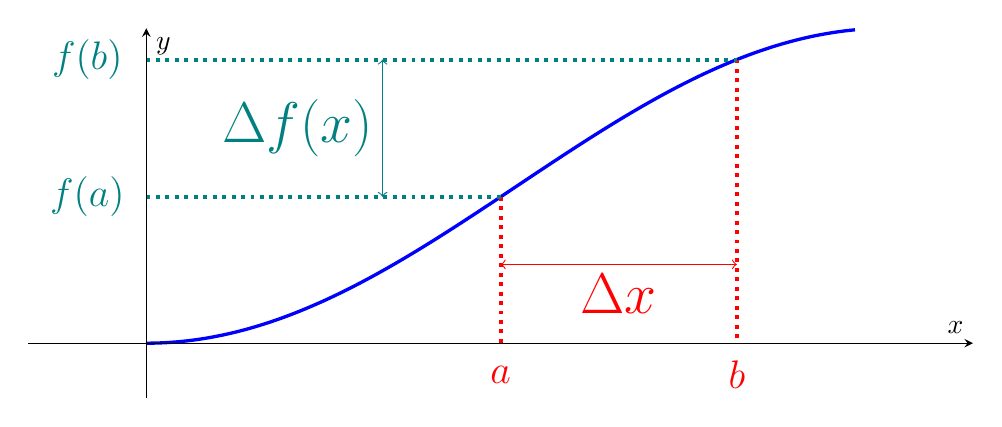
\begin{tikzpicture}
    \begin{axis}[
        axis on top,axis lines=center,
        xlabel={$x$}, 
        ylabel={$y$},
        ymin=-0.7, ymax=4,
        xmin=-0.5, xmax=3.5,
        x=3cm,
        y=1cm,
        xtick=\empty,
        ytick=\empty,
        %grid=both,
     %xmajorgrids={true}
        %major grid style={black!50}
    ] \addplot+[samples=501,very thick,smooth,blue,domain=0:3, no marks] {-2*cos(deg(x))+2};
    \draw[red,dotted,line width=0.5mm] (axis cs:1.5,{-2*cos(deg(1.5))+2}) -- (axis cs:1.5,0);
    \draw[teal,dotted,line width=0.5mm] (axis cs:0,{-2*cos(deg(1.5))+2}) -- (axis cs:1.5,{-2*cos(deg(1.5))+2});
    \node[red] at (axis cs:1.5,-0.4) {\Large{$a$}};
    \node[teal] at (axis cs:-0.25,{-2*cos(deg(1.5))+2}) {\Large{$f(a)$}};
    \draw[red,dotted,line width=0.5mm] (axis cs:2.5,{-2*cos(deg(2.5))+2}) -- (axis cs:2.5,0);
    \draw[teal,dotted,line width=0.5mm] (axis cs:0,{-2*cos(deg(2.5))+2}) -- (axis cs:2.5,{-2*cos(deg(2.5))+2});
    \node[red] at (axis cs:2.5,-0.4) {\Large{$b$}};
    \node[teal] at (axis cs:-0.25,{-2*cos(deg(2.5))+2}) {\Large{$f(b)$}};
    \draw[red,<->] (axis cs:1.5,1) -- (axis cs:2.5,1) node [red,midway,below] {\huge{$\Delta x$}};
    \draw[teal,<->] (axis cs:1,{-2*cos(deg(1.5))+2}) -- (axis cs:1,{-2*cos(deg(2.5))+2}) node [teal,midway,left] {\huge{$\Delta f(x)$}};
    \end{axis}
\end{tikzpicture}
\end{image}

Deze verhouding noemen we het \textbf{differentiequotiënt}.
\end{definitie}


\begin{voorbeeld}

Beschouw

\[
f(x)=-x^2+8x.
\]

Bepaal de gemiddelde verandering over $[2,4]$.

\begin{oplossing}[toon]

  \begin{center}
    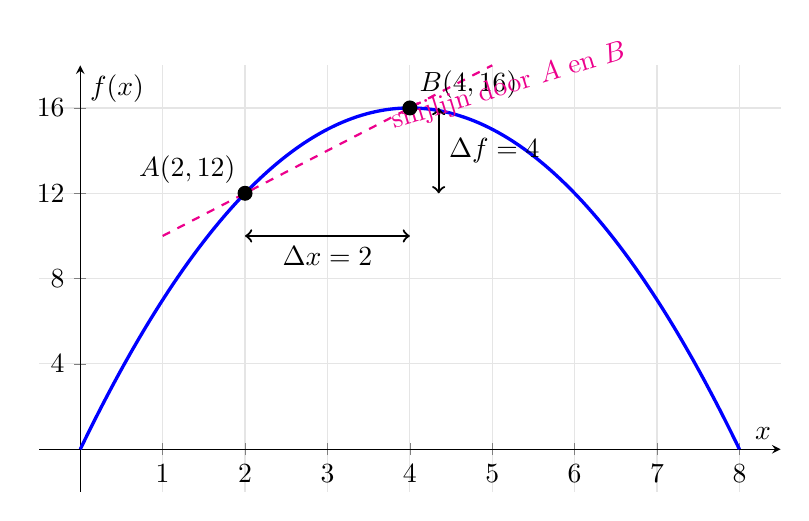
\begin{tikzpicture}
    \begin{axis}[
        axis lines=middle,
        xmin=-0.5, xmax=8.5,
        ymin=-2, ymax=18,
        width=11cm,
        height=7cm,
        xlabel={$x$},
        ylabel={$f(x)$},
        xtick={0,1,...,8},
        ytick={0,4,8,12,16},
        grid=major,
        grid style={gray!20},
        samples=200,
        domain=0:8,
        clip=false
    ]
    
    % Grafiek van de functie
    \addplot[
        blue,
        very thick
    ]
    {-x^2+8*x};
    
    % Snijlijn door A en B: y = 2x + 8
    \addplot[
        magenta,
        thick,
        dashed,
        domain=1:5
    ]
    {2*x+8};
    
    % Punten A en B
    \addplot[
        only marks,
        mark=*,
        mark size=2.5pt
    ]
    coordinates {(2,12) (4,16)};
    
    \node[above left] at (axis cs:2,12) {$A(2,12)$};
    \node[above right] at (axis cs:4,16) {$B(4,16)$};
    
    % Horizontale en verticale verandering
    \draw[<->, thick]
        (axis cs:2,10) -- node[below] {$\Delta x=2$} (axis cs:4,10);
    
    \draw[<->, thick]
        (axis cs:4.35,12) -- node[right] {$\Delta f=4$} (axis cs:4.35,16);
    
    % Label snijlijn
    \node[magenta, rotate=17] at (axis cs:5.2,17)
        {snijlijn door $A$ en $B$};
    
    \end{axis}
    \end{tikzpicture}
    \end{center}

We berekenen eerst

\[
f(2)=-2^2+8\cdot2=12
\]

en

\[
f(4)=-4^2+8\cdot4=16.
\]

Daarom is

\[
\frac{f(4)-f(2)}{4-2}
=
\frac{16-12}{2}
=
2.
\]

De functiewaarde neemt tussen $x=2$ en $x=4$
\textbf{gemiddeld met $2$ eenheden toe per eenheid toename van $x$}.

\end{oplossing}

\end{voorbeeld}


\begin{oefening}[Gemiddelde verandering]{\oefB \ESS}

Voor een functie $f$ geldt

\[
f(3)=7
\qquad\text{en}\qquad
f(8)=2.
\]

Bereken de gemiddelde verandering over $[3,8]$.

\[
\frac{f(8)-f(3)}{8-3}
=
\answer{-1}.
\]

Welke interpretatie is correct?

\begin{multipleChoice}
  \choice{De functie daalt overal met precies $1$.}
  \choice[correct]{Tussen $x=3$ en $x=8$ neemt de functiewaarde
  gemiddeld met $1$ af per eenheid toename van $x$.}
  \choice{De functiewaarde is gelijk aan $-1$.}
  \choice{Elke raaklijn aan de grafiek heeft richtingscoëfficiënt $-1$.}
\end{multipleChoice}

\end{oefening}


%%%%%%%%%%%%%%%%%%%%%%%%%%%%%%%%%%%%%%%%%%%%%%%%%%%%%%%%%%%%%%%%%%%%%%
%% snijlijn
%%%%%%%%%%%%%%%%%%%%%%%%%%%%%%%%%%%%%%%%%%%%%%%%%%%%%%%%%%%%%%%%%%%%%%

\FVDsubsection{Meetkundige betekenis}

Beschouw de punten

\[
A(a,f(a))
\qquad\text{en}\qquad
B(b,f(b))
\]

op de grafiek van $f$.

De rechte door $A$ en $B$ is een \textbf{snijlijn}.

De richtingscoëfficiënt van deze snijlijn is

\[
\operatorname{rico}(AB)
=
\frac{f(b)-f(a)}{b-a}.
\]

Dat is precies het differentiequotiënt.

\begin{definitie}[]
Het differentiequotiënt is de
\textbf{richtingscoëfficiënt van de snijlijn}
door de twee overeenkomstige punten van de grafiek.

\[
\important{
\text{gemiddelde verandering}
\longleftrightarrow
\text{richtingscoëfficiënt van een snijlijn}
}
\]

\begin{image}
  \begin{tikzpicture}[scale=0.75]
    \begin{axis}[
        axis on top,axis lines=center,
        xlabel={$x$}, 
        ylabel={$y$},
        ymin=-0.7, ymax=6.2,
        xmin=-0.5, xmax=6,
        x=2cm,
        y=1cm,
        xtick=\empty,
        ytick=\empty,
        %grid=both,
        %xmajorgrids={true}
        %major grid style={black!50}
    ] \addplot+[samples=501,very thick,smooth,blue,domain=0:5, no marks] {-(x-3)*(x-3)+6};
    \draw[red,dotted,line width=0.5mm] (axis cs:1,0) -- (axis cs:1,2);
    \draw[teal,dotted,line width=0.5mm] (axis cs:0,2) -- (axis cs:1,2);
    \node[red] at (axis cs:1,-0.4) {\Large{$a$}};
    \node[teal] at (axis cs:-0.25,2) {\Large{$f(a)$}};
    \draw[red,fill=red,thick] (axis cs:1,2) circle (0.1cm) node[orange, anchor=north west]{\Large{$A$}};
    \draw[red,dotted,line width=0.5mm] (axis cs:4,0) -- (axis cs:4,5);
    \draw[teal,dotted,line width=0.5mm] (axis cs:0,5) -- (axis cs:4,5);
    \node[red] at (axis cs:4,-0.4) {\Large{$b$}};
    \node[teal] at (axis cs:-0.25,5) {\Large{$f(b)$}};
    \draw[red,fill=red,thick] (axis cs:4,5) circle (0.1cm) node[orange, anchor=north east]{\Large{$B$}};
    \addplot+[samples=501,very thick,smooth,red,domain=0.5:5, no marks] {x+1};
    \node[red] at (axis cs: 5.2, 5.2) {\Large{$rico \ AB=\dfrac{\Delta f}{\Delta x}$}};
    \end{axis}
\end{tikzpicture}
\end{image}
\end{definitie}





%%%%%%%%%%%%%%%%%%%%%%%%%%%%%%%%%%%%%%%%%%%%%%%%%%%%%%%%%%%%%%%%%%%%%%
%% OGENBLIKKELIJKE VERANDERING
%%%%%%%%%%%%%%%%%%%%%%%%%%%%%%%%%%%%%%%%%%%%%%%%%%%%%%%%%%%%%%%%%%%%%%

\FVDsection{Van gemiddelde naar ogenblikkelijke verandering}

\FVDsubsection{Het interval steeds kleiner maken}

We kiezen een vast punt

\[
A(a,f(a))
\]

op de grafiek van $f$.

Daarnaast nemen we een tweede punt

\[
B(F,f(x)).
\]

Voor $x\neq a$ heeft de snijlijn $AB$ richtingscoëfficiënt

\[
\frac{f(x)-f(a)}{x-a}.
\]

Nu laten we $x$ steeds dichter bij $a$ komen:

\[
x\to a.
\]

Het punt $B$ nadert dan tot $A$.
\begin{image}[\textwidth]
  \begin{tikzpicture}
 \begin{axis}[
     axis on top,axis lines=center,
     xlabel={$x$}, 
     ylabel={$y$},
     ymin=-0.7, ymax=6.2,
     xmin=-0.5, xmax=6,
     x=2cm,
     y=1cm,
     xtick=\empty,
     ytick=\empty,
     %grid=both,
     %xmajorgrids={true}
     %major grid style={black!50}
 ] \addplot+[samples=501,very thick,smooth,blue,domain=0:5, no marks] {-(x-3)*(x-3)+6};
 \addplot+[samples=501,very thick,smooth,purple,domain=0:5, no marks] {4*x-2} node[purple] at (axis cs: 1.25,5.5) {{raaklijn $t$}};
 \draw[red,dotted,line width=0.5mm] (axis cs:1,0) -- (axis cs:1,2);
 \draw[teal,dotted,line width=0.5mm] (axis cs:0,2) -- (axis cs:1,2);
 \node[red] at (axis cs:1,-0.4) {\large{$a$}};
 \node[teal] at (axis cs:-0.25,2) {\large{$f(a)$}};
 \draw[red,fill=red,thick] (axis cs:1,2) circle (0.1cm) node[orange, anchor=north west]{\large{$A$}};
 \draw[red,dotted,line width=0.5mm] (axis cs:4,0) -- (axis cs:4,5);
 \draw[teal,dotted,line width=0.5mm] (axis cs:0,5) -- (axis cs:4,5);
 \node[red] at (axis cs:4,-0.4) {\large{$x$}};
 \node[teal] at (axis cs:-0.25,5) {\large{$f(x)$}};
 \draw[red,fill=red,thick] (axis cs:4,5) circle (0.1cm) node[orange, anchor=north east]{\large{$B$}};
 \addplot+[samples=501,very thick,smooth,red,domain=0.5:5, no marks] {x+1};
 \node[red] at (axis cs: 5.2, 5.2) {\large{$rico \ AB=\dfrac{\Delta f}{\Delta x}$}};
 \draw[teal,->] (axis cs:1,2) -- (axis cs: 4,2) node[teal,midway,below] {\large{$\Delta x=x-a$}};
 \draw[teal,->] (axis cs:4,2) -- (axis cs: 4,5) node[teal,midway,right] {\large{$\Delta f=f(x)-f(a)$}}
 ;
 \end{axis}
\end{tikzpicture}
\end{image} 
De snijlijn door $A$ en $B$ nadert naar de raaklijn aan de grafiek
in $A$.

We onderzoeken daarom

\[
\lim_{x\to a}
\frac{f(x)-f(a)}{x-a}.
\]

Deze limiet beschrijft niet langer een gemiddelde verandering
over een interval, maar de \textbf{ogenblikkelijke verandering}
bij $x=a$.


%%%%%%%%%%%%%%%%%%%%%%%%%%%%%%%%%%%%%%%%%%%%%%%%%%%%%%%%%%%%%%%%%%%%%%
%% AFGELEID GETAL
%%%%%%%%%%%%%%%%%%%%%%%%%%%%%%%%%%%%%%%%%%%%%%%%%%%%%%%%%%%%%%%%%%%%%%

\FVDsection{Het afgeleid getal}

\begin{definitie}[Afgeleid getal]
Als de limiet

\[
\lim_{x\to a}
\frac{f(x)-f(a)}{x-a}
\]

bestaat en een reëel getal is, dan is $f$
\textbf{afleidbaar in $a$}.

Het \textbf{afgeleid getal van $f$ in $a$} is

\[
\important{
f'(a)
=
\lim_{x\to a}
\frac{f(x)-f(a)}{x-a}
}.
\]
\end{definitie}

We kunnen dezelfde definitie schrijven met

\[
x=a+h.
\]

Wanneer $x\to a$, geldt $h\to0$.

Daarom is ook

\[
\important{
f'(a)
=
\lim_{h\to0}
\frac{f(a+h)-f(a)}{h}
}.
\]



\begin{voorbeeld}

Gegeven is

\[
f(x)=x^2+2x.
\]

Bepaal $f'(1)$ met de definitie.

\begin{oplossing}

We gebruiken

\[
f'(1)
=
\lim_{x\to1}
\frac{f(x)-f(1)}{x-1}.
\]

Omdat

\[
f(1)=3,
\]

volgt

\begin{align*}
f'(1)
&=
\lim_{x\to1}
\frac{x^2+2x-3}{x-1}
\\
&=
\lim_{x\to1}
\frac{(x-1)(x+3)}{x-1}
\\
&=
\lim_{x\to1}(x+3)
\\
&=4.
\end{align*}

Dus

\[
\boxed{f'(1)=4}.
\]

\end{oplossing}

\end{voorbeeld}

De berekening is slechts één deel van het antwoord.

De waarde

\[
f'(1)=4
\]

betekent ook dat de ogenblikkelijke verandering van $f$
bij $x=1$ gelijk is aan $4$.


\FVDsubsection{Meetkundige betekenis}

De overgang van snijlijn naar raaklijn geeft onmiddellijk de
meetkundige betekenis van het afgeleid getal.

\begin{definitie}[Betekenis afgeleid getal]
Het afgeleid getal $f'(a)$ is de
\textbf{richtingscoëfficiënt van de raaklijn}
aan de grafiek van $f$ in het punt

\[
P(a,f(a)).
\]

Dus

\[
\important{
f'(a)=\operatorname{rico}(t)
}
\]

waarbij $t$ de raaklijn is in $P$.
\begin{image}
  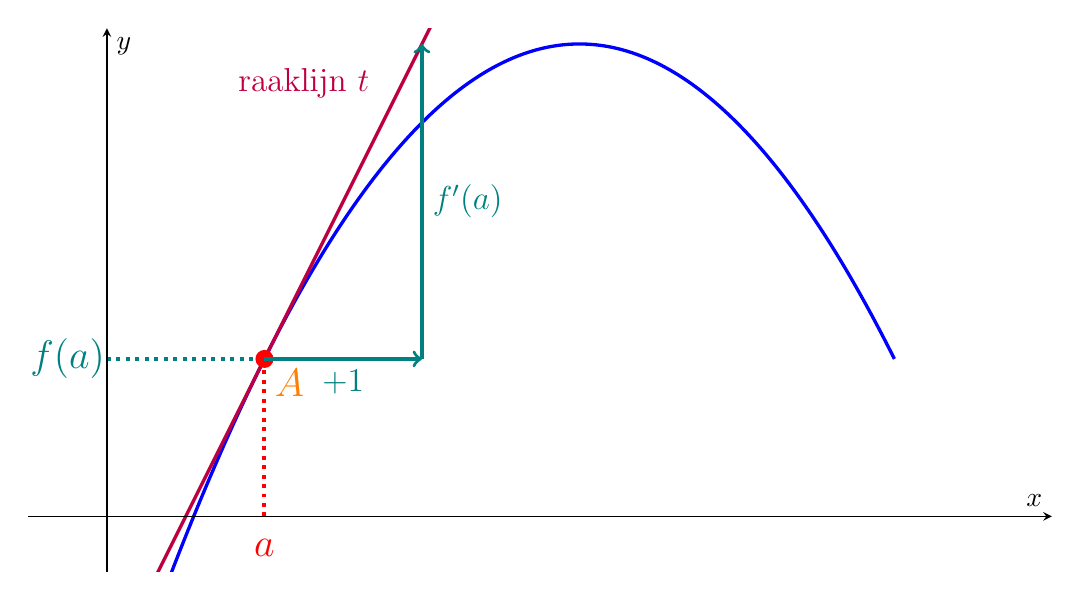
\begin{tikzpicture}
                      \begin{axis}[
                          axis on top,axis lines=center,
                          xlabel={$x$}, 
                          ylabel={$y$},
                          ymin=-0.7, ymax=6.2,
                          xmin=-0.5, xmax=6,
                          x=2cm,
                          y=1cm,
                          xtick=\empty,
                          ytick=\empty,
                          %grid=both,
                          %xmajorgrids={true}
                          %major grid style={black!50}
                      ] \addplot+[samples=501,very thick,smooth,blue,domain=0:5, no marks] {-(x-3)*(x-3)+6};
                      \addplot+[samples=501,very thick,smooth,purple,domain=0:5, no marks] {4*x-2} node[purple] at (axis cs: 1.25,5.5) {\large{raaklijn $t$}};
                      \draw[red,dotted,line width=0.5mm] (axis cs:1,0) -- (axis cs:1,2);
                      \draw[teal,dotted,line width=0.5mm] (axis cs:0,2) -- (axis cs:1,2);
                      \node[red] at (axis cs:1,-0.4) {\Large{$a$}};
                      \node[teal] at (axis cs:-0.25,2) {\Large{$f(a)$}};
                      \draw[red,fill=red,thick] (axis cs:1,2) circle (0.1cm) node[orange, anchor=north west]{\Large{$A$}};
                      \draw[teal,->,very thick] (axis cs:1,2) -- (axis cs: 2,2) node[teal,midway,below] {\large{$+1$}};
                      \draw[teal,->,very thick] (axis cs:2,2) -- (axis cs: 2,6) node[teal,midway,right] {\large{$f'(a)$}}
                      ;
                      \end{axis}
                  \end{tikzpicture}
\end{image}
\end{definitie}


\FVDsubsection{Wat vertelt het teken?}

Als

\[
f'(a)>0,
\]

heeft de raaklijn een positieve richtingscoëfficiënt.

Als

\[
f'(a)<0,
\]

heeft de raaklijn een negatieve richtingscoëfficiënt.

Als

\[
f'(a)=0,
\]

is de raaklijn horizontaal.

\begin{opmerking}
Uit

\[
f'(a)=0
\]

mag je niet onmiddellijk besluiten dat $f$ in $a$
een maximum of minimum bereikt.

Een horizontale raaklijn is op zichzelf onvoldoende om een
extremum te besluiten.
\end{opmerking}




\begin{oefening}[Concentratie verandering]{\oefB \ESS}

De functie $C(t)$ beschrijft een concentratie in $\mathrm{mg/L}$,
waarbij $t$ wordt uitgedrukt in minuten.

Er geldt

\[
C'(12)=-0,30.
\]

Welke interpretatie is correct?

\begin{multipleChoice}

\choice{
Na $12$ minuten bedraagt de concentratie
$-0,30~\mathrm{mg/L}$.
}

\choice{
Gedurende de eerste $12$ minuten daalt de concentratie
gemiddeld met $0,30~\mathrm{mg/L}$.
}

\choice[correct]{
Op het tijdstip $t=12$ minuten neemt de concentratie
ogenblikkelijk af met $0,30~\mathrm{mg/L}$ per minuut.
}

\choice{
Na $12$ minuten is de concentratie nul.
}

\end{multipleChoice}

\end{oefening}


%%%%%%%%%%%%%%%%%%%%%%%%%%%%%%%%%%%%%%%%%%%%%%%%%%%%%%%%%%%%%%%%%%%%%%
%% RAAKLIJNVERGELIJKING
%%%%%%%%%%%%%%%%%%%%%%%%%%%%%%%%%%%%%%%%%%%%%%%%%%%%%%%%%%%%%%%%%%%%%%

\FVDsubsection{De vergelijking van de raaklijn}

De raaklijn aan de grafiek in

\[
P(a,f(a))
\]

heeft richtingscoëfficiënt

\[
f'(a).
\]

Een rechte met richtingscoëfficiënt $m$ door een punt
$(x_1,y_1)$ heeft vergelijking

\[
y-y_1=m(x-x_1).
\]

Daaruit volgt:

\begin{definitie}[De raaklijn]
De raaklijn aan de grafiek van $f$ in het punt
$P(a,f(a))$ heeft vergelijking

\[
\important{
y-f(a)=f'(a)(x-a)
}.
\]
\end{definitie}


\begin{voorbeeld}

Gegeven is

\[
f(x)=x^2+2x.
\]

We weten dat

\[
f(1)=3
\qquad\text{en}\qquad
f'(1)=4.
\]

De raaklijn bij $x=1$ heeft dus vergelijking

\begin{align*}
y-3 &= 4(x-1)
\\
y-3 &= 4x-4
\\
y &= 4x-1.
\end{align*}

Dus

\[
\boxed{y=4x-1}.
\]

\end{voorbeeld}


\begin{oefening} {\oefB \ESS}

Voor een functie $f$ geldt

\[
f(2)=5
\qquad\text{en}\qquad
f'(2)=-3.
\]

Vul aan.

De raaklijn gaat door

\[
P=(\answer{2},\answer{5})
\]

en heeft richtingscoëfficiënt

\[
\answer{-3}.
\]

De vergelijking is

\[
y-5=-3(x-2),
\]

dus

\[
y=\answer{-3}x+\answer{11}.
\]

\end{oefening}


%%%%%%%%%%%%%%%%%%%%%%%%%%%%%%%%%%%%%%%%%%%%%%%%%%%%%%%%%%%%%%%%%%%%%%
%% VERBANDEN
%%%%%%%%%%%%%%%%%%%%%%%%%%%%%%%%%%%%%%%%%%%%%%%%%%%%%%%%%%%%%%%%%%%%%%

\FVDsection{Drie talen van de afgeleide}

Eenzelfde uitspraak over een afgeleide kunnen we op verschillende
manieren formuleren.

\begin{center}
\begin{tabular}{p{0.25\textwidth}|p{0.62\textwidth}}
\textbf{Algebraïsch}
&
$f'(a)$ is de limiet van de differentiequotiënten.
\\[2mm]

\textbf{Meetkundig}
&
$f'(a)$ is de richtingscoëfficiënt van de raaklijn bij $x=a$.
\\[2mm]

\textbf{In context}
&
$f'(a)$ beschrijft de ogenblikkelijke verandering van de
afhankelijke grootheid bij $x=a$.
\end{tabular}
\end{center}

Bij analyse moet je tussen deze drie voorstellingen kunnen schakelen.





\FVDsection{Samengevat}

Over een interval $[a,b]$ gebruiken we het differentiequotiënt

\[
\boxed{
\frac{f(b)-f(a)}{b-a}
}.
\]

Dit beschrijft de gemiddelde verandering en is de
richtingscoëfficiënt van een snijlijn.

Bij één punt gebruiken we het afgeleid getal

\[
\boxed{
f'(a)
=
\lim_{x\to a}
\frac{f(x)-f(a)}{x-a}
}.
\]

Dit beschrijft de ogenblikkelijke verandering en is de
richtingscoëfficiënt van de raaklijn bij $x=a$.

De vergelijking van die raaklijn is

\[
\boxed{
y-f(a)=f'(a)(x-a)
}.
\]

Bij toepassingen interpreteren we een afgeleid getal altijd
in functie van de grootheden, het teken en de eenheden.


\begin{oefening}[Alle begrippen samen] {\oefB \ESS}

Van een functie $f$ weten we dat

\[
f(2)=7
\qquad\text{en}\qquad
f'(2)=-3.
\]

\begin{question}

Door welk punt gaat de raaklijn?

\[
P=(\answer{2},\answer{7}).
\]

\end{question}

\begin{question}

Wat is de richtingscoëfficiënt van de raaklijn?

\[
\operatorname{rico}(t)=\answer{-3}.
\]

\end{question}

\begin{question}

Hoe verloopt de raaklijn van links naar rechts?

\begin{multipleChoice}
  \choice{Ze stijgt.}
  \choice[correct]{Ze daalt.}
  \choice{Ze is horizontaal.}
\end{multipleChoice}

\end{question}

\begin{question}

Bepaal de vergelijking van de raaklijn.

\[
y-7=-3(x-2),
\]

dus

\[
y=\answer{-3}x+\answer{13}.
\]

\end{question}

\begin{question}

Een leerling beweert:

\begin{center}
``Omdat $f'(2)=-3$, geldt noodzakelijk $f(3)=4$.''
\end{center}

Is dat correct?

\begin{multipleChoice}

\choice{
Ja, want $7-3=4$.
}

\choice[correct]{
Nee. $f'(2)$ beschrijft de ogenblikkelijke verandering bij $x=2$.
Daaruit volgt niet dat de functie over het volledige interval
$[2,3]$ met precies $3$ afneemt.
}

\end{multipleChoice}

\end{question}

\end{oefening}







\end{document}